\headline{{\textbf{\Large\sffamily Bonsai Roots:}}\\
          {\textbf{\large\sffamily Meet the Members of TWBC}}}
\label{2024-12-roots}
\noindent
Welcome to our revived monthly column, \emph{Bonsai Roots}, where we get to know the members of the Twickenham Bonsai Club a little better.
% Each month, we'll feature one of our members, sharing their bonsai journey, insights, and aspirations.
This column aims to strengthen connections within our club and give potential new members a glimpse into the vibrant community we've built.
Our first feature is \textbf{Stefano}.
%, a new member whose enthusiasm for bonsai and engaging story truly capture the spirit of the TWBC.

\begin{window}[%
    0,l,%
    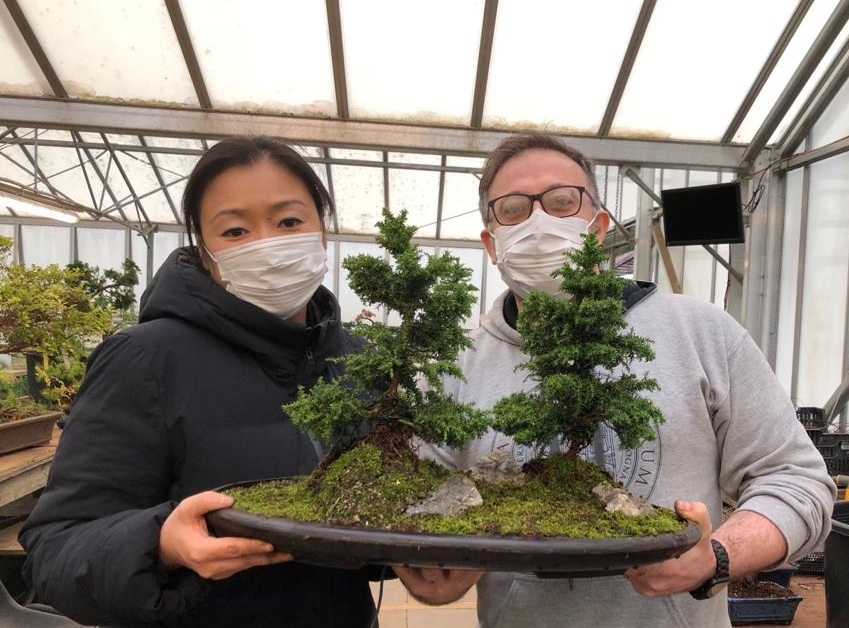
\includegraphics[width=1.0\columnwidth]{2024_12/res/roots.jpg},%
    \centerline{\emph{Stefano and Yoshie at Herons Bonsai.}}%
]
    \begin{itemize}
        \item \textbf{What's your name and where in the country do you live?}

        \emph{Hi, I'm Stefano. I've lived in the UK for the past 12 years and currently reside in Southfields, London, with my partner Yoshie and our dog Kuma.}

        \item \textbf{What are your favourite species of tree and why?}

        \emph{I love pines and larches because they remind me of childhood holidays in the Alps. I also adore deciduous trees, especially Japanese maples, for their elegance, and ficuses, which grow quickly and are rewarding to work on all year round.}

        \item \textbf{What aspect of bonsai do you enjoy?}

        \emph{Bonsai calms my nerves and relieves stress. It also allows me to express my artistic side, which my job doesn't often accommodate.}

        \item \textbf{What aspects of bonsai do you find most challenging?}

        \emph{Styling trees from scratch is where I struggle most. I've learned the horticultural side of bonsai, but shaping and refining a tree is still a challenge.}

        \item \textbf{Who or what inspires you throughout your bonsai journey?}

        \emph{I try to stay open-minded and take inspiration from everything I see. Experienced bonsai practitioners are a huge influence, but I also learn by trying out anything I find interesting or challenging.}

        \item \textbf{How long have you been interested in keeping bonsai?}

        \emph{I've been fascinated by bonsai for about four years, ever since Yoshie gifted me a Chinese Elm for my birthday during the pandemic.}

        \item \textbf{What stimulated your interest in bonsai?}

        \emph{Like many others, my first exposure to bonsai came from The Karate Kid during my teenage years. That initial fascination lay dormant until I received my first tree, which reignited my passion.}

        \item \textbf{If you could give someone new to bonsai any tips, what would it be?}

        \emph{Do what makes you happy! Enjoyment keeps you motivated, and over time, you'll naturally start seeking ways to improve.}

        \item \textbf{Why do you enjoy being part of TWBC, and do you have any ideas or suggestions for the club's future?}

        \emph{I've always wanted to join a bonsai club, and I'm loving it so far! I look forward to bringing my trees to club nights for feedback and suggestions. One idea I have is to publish a club website to make it easier for new members to find us.}

        \item \textbf{One word to describe what bonsai means to you?}

        \emph{Peace of mind.}

        \item \textbf{What are your future goals regarding your own trees and learning more about the hobby?}

        \emph{I'd like to grow elegant bonsai from seeds and cuttings, particularly Shohin and Mame due to limited space. My current focus is learning the fundamentals of bonsai and developing my own style.}

        \item \textbf{How would you like to see your bonsai journey progress in the future?}

        \emph{I hope to create trees that are worthy of being displayed, so my love for nature and my effort into this art is recognized.}

    \end{itemize}
\end{window}

We hope you enjoyed Stefano's inspiring story.
Who will we meet next month?
Stay tuned for more from \emph{Bonsai Roots}!

\closearticle
